\title{Lab Four: Shift registers and counters}
\author{Ben Smith}

%| This is a header file for Latex documents  
%| It contains a number of common packages, settings, and custom macros that I frequently use.
\documentclass[9pt,journal]{IEEEtran}

\usepackage[cmex10]{amsmath}        %| American Mathematical Society package for fancy maths  b
\interdisplaylinepenalty=2500              %| Restores IEEE line spacing after amsmath

%| IEEE Citation package
\usepackage{cite}
\usepackage[section]{placeins}
\usepackage{array}
\usepackage{dblfloatfix}
\usepackage{color}
\usepackage{graphicx}
\usepackage{float}
\usepackage{url}                         %| Improved URL handling
\usepackage{etoolbox}
\usepackage[font=footnotesize]{subcaption}
\usepackage{listings}
\usepackage{fixltx2e}               %| Better tables than for LaTeX 2e
\usepackage{minted}

%| Highlighting for source code listings
\definecolor{mygreen}{rgb}{0,0.6,0}
\definecolor{ltgray}{rgb}{0.93,0.93,0.93}
\definecolor{dkgray}{rgb}{0.5,0.5,0.5}
\definecolor{mymauve}{rgb}{0.58,0,0.82}
\lstset{
  backgroundcolor=\color{ltgray},  % choose the background color; you must add \usepackage{color} or \usepackage{xcolor}
  basicstyle=\scriptsize\ttfamily, % the size of the fonts that are used for the code
  breakatwhitespace=true,         % sets if automatic breaks should only happen at whitespace
  breaklines=true,                 % sets automatic line breaking
  captionpos=b,                    % sets the caption-position to bottom
  commentstyle=\color{mygreen},    % comment style
  deletekeywords={...},            % if you want to delete keywords from the given language
  escapeinside={\%*}{*)},          % if you want to add LaTeX within your code
  extendedchars=true,              % lets you use non-ASCII characters; for 8-bits encodings only, does not work with UTF-8
  frame=single,                    % adds a frame around the code
  keepspaces=true,                 % keeps spaces in text, useful for keeping indentation of code (possibly needs columns=flexible)
  keywordstyle=\color{blue},       % keyword style
  language=SystemVerilog,          % the language of the code(I modified the .sty for systemverilog, found the code on google)
  morekeywords={*,...},            % if you want to add more keywords to the set
  numbers=left,                    % where to put the line-numbers; possible values are (none, left, right)
  numbersep=4pt,                   % how far the line-numbers are from the code
  numberstyle=\tiny\color{dkgray}, % the style that is used for the line-numbers
  rulecolor=\color{black},         % if not set, the frame-color may be changed on line-breaks within not-black text (e.g. comments (green here))
  showspaces=false,                % show spaces everywhere adding particular underscores; it overrides 'showstringspaces'
  showstringspaces=false,          % underline spaces within strings only
  showtabs=false,                  % show tabs within strings adding particular underscores
  stepnumber=2,                    % the step between two line-numbers. If it's 1, each line will be numbered
  stringstyle=\color{mymauve},     % string literal style
  tabsize=2,                       % sets default tabsize to 2 spaces
  title=\lstname                   % show the filename of files included with \lstinputlisting; also try caption instead of title
}

\lstset{keywordstyle=\color{purple}}
\lstset{keywordstyle={[2]\color{purple}} }
\lstset{keywordstyle={[3]\color{magenta}} }
\lstset{keywordstyle={[4]\color{teal} }}
\lstset{keywordstyle={[5]\color{violet!40}} }

% Alter some LaTeX defaults for better treatment of figures:
  % See p.105 of ''TeX Unbound'' for suggested values.
  % See pp. 199-200 of Lamport's ''LaTeX'' book for details.
  %   General parameters, for ALL pages:
  \renewcommand{\topfraction}{0.9}  % max fraction of floats at top
  \renewcommand{\bottomfraction}{0.8} % max fraction of floats at bottom
  %   Parameters for TEXT pages (not float pages):
  \setcounter{topnumber}{2}
  \setcounter{bottomnumber}{2}
  \setcounter{totalnumber}{4}     % 2 may work better
  \setcounter{dbltopnumber}{2}    % for 2-column pages
  \renewcommand{\dbltopfraction}{0.9} % fit big float above 2-col. text
  \renewcommand{\textfraction}{0.07}  % allow minimal text w. figs
  %   Parameters for FLOAT pages (not text pages):
  \renewcommand{\floatpagefraction}{0.7}  % require fuller float pages
  % N.B.: floatpagefraction MUST be less than topfraction !!
  \renewcommand{\dblfloatpagefraction}{0.7} % require fuller float pages

%| Enables PDF metadata, thumbnails, and navigation
\newcommand\MYhyperrefoptions{
  bookmarks=true,
  bookmarksnumbered=true,
  pdfpagemode={UseOutlines},
  plainpages=false,
  pdfpagelabels=true,
  colorlinks=true,
  linkcolor={black},
  citecolor={black},
  urlcolor={blue},
  pdftitle={CPE/EEE 64 Lab},
  pdfsubject={Engineering},                        
  pdfauthor={Ben Smith},
  pdfkeywords={Logic Design, FPGA, Verilog}}                       

%| Calls hyperref package with the options specified above
\usepackage[\MYhyperrefoptions,pdftex]{hyperref}

%| Font settings
\renewcommand{\sfdefault}{phv}
\renewcommand{\rmdefault}{ptm}
\renewcommand{\ttdefault}{pcr}

%| Restores IEEE table formatting after usage of subcaption package
\captionsetup[table]{format=plain,labelformat=simple,justification=centering, labelsep=newline, singlelinecheck=false, textfont={sc}}

%| Required Lab Demo custom function
%| \demo{Name}{Physical deliverable}{Documentation deliverable}{Process}
%| =================================================================================================
%| for boxed text and stuch
\usepackage{fancybox}
\newenvironment{fminipage}%
{\begin{Sbox}\begin{minipage}}%
{\end{minipage}\end{Sbox}\Ovalbox{\TheSbox}}

%| Actual bawx
\newcommand{\demo}[4] {
\vspace{15px}
\begin{centering}
  \begin{fminipage}{.47\textwidth}
    \vspace{3px}
    \centering{\bfseries \large Laboratory Demo: #1}\\*
    \vspace{10px}
    \begin{tabular}{p{1.4cm}  p{6.3cm}}
      %|==Requirements for lab demo==
      \raggedright Specification:                  &#2\\
      \\
      \raggedright  Deliverable:                   &#3\\
      \\
      \raggedright Process :                       &#4\\
    \end{tabular}
  \end{fminipage}
\end{centering}
}

%| Single figure
%| \small{Location}{Caption}{Label}
%| =================================================================================================
\newcommand{\smallfig}[3] {
  \begin{figure}[H]
    \includegraphics[width=.48\textwidth]{#1}
    \caption{#2}
    \label{#3}
  \end{figure}
}

%| Single figure
%| \simpletable{c||c}{Caption}{Label}{content}
%| =================================================================================================
\newcommand{\simpletable}[4] {
  \begin{table}[!t]
    \caption{#2}
    \label{#3}
    \centering
    \begin{tabular}{#1}
      \hline
      #4
    \end{tabular}
  \end{table}
}
\begin{document}

  \maketitle
    \begin{abstract}
      This document introduces concepts related to the implementation of Registers and Timers in the System Verilog hardware descriptive language. The effects of register timing, metastability and the FPGA timing closure process are breifly discussed.
    \end{abstract}
%| =================================================================================================
%| Introduction
%| =================================================================================================
\section{Introduction}
  \PARstart{T}{his} lab will reinforce the idea of modularity as we design modules which depend on a clocking signal. Clocking circuits allows the synchronization of large blocks of logic. The concepts this lab introduces are at the core of design with Verilog. The sensitivity list will allow you to communicate with a number of different devices on different system clocks greatly expanding the usefulness of the FPGA. It is important to remember that each one of these blocks evaluates simultaneously, the behavioral block is at the core of Verilog's parallel nature. The purpose of this lab is to introduce the following concepts:
    \begin{itemize}
      \item Using synchronous logic with a system clock
      \item The implications of timing constraints
    \end{itemize}
    

  %| Clocked designs in Verilog
  %| =================================================================================================
  \subsection{Clocked designs in Verilog}

    \subsubsection{Posedge and Negedge in the sensitivity list}
      These operators are commonly used in the sensitivity list of a logical block in Verilog. They indicate where operations are performed on a square wave clock signal. Posedge performs the specified operation at the low to high transition and negedge the high to low edge.
    
    \subsubsection{Register metastability and timing closure}
      ``Timing Closure'' is the process of making sure the physical circuits on the FPGA (or any digital system) and produce a desired functionality. The electrical properties of capacitance and inductance limit the maximum operating frequency of a circuit, even on the nanometer scale on the FPGA. The systems that are built in this lab do not approach the abilities of the Cyclone FPGA we are using. But the topic is very important, it has been one of the first questions I have been asked on a job interview. If you would like to learn about the topic (not required) Altera's white paper \href{http://www.altera.com/literature/wp/wp-01082-quartus-ii-metastability.pdf}{01082} offers a technical discussion of metastability and how to mitigate the effects of the phenomenon.

  %| Blocking and non blocking operators
  %| =================================================================================================
  \subsection{Blocking and non blocking operators}
    Verilog statements can be structured by using two different assignments. These two types of statements must be used to avoid race conditions when your code is synthesized. Once again Clifford Cummings offers a great insight into the operation of these language constructs. 
      
    \subsubsection{Blocking assignments \bfseries ( = )} 
      Blocking assignments occur in one step, all other operations are ``paused'' while waiting for the operation to complete.Evaluate the RHS (right-hand side equation) and update the LHS (left-hand side expression) of the blocking assignment without interruption from any other Verilog statement.''\cite{Sunburst:BlockNoBlock}

    \subsubsection{Non-Blocking assignments \bfseries ( $<$= )} 
      The evaluation of nonblocking assignments is a bit more complex than the blocking operator and requires special consideration. The execution of these statements is defined as follows. This information is particularly relevant in the simulator as you try to debug your design. \cite{Sunburst:BlockNoBlock} 
      \begin{enumerate}
        \item Evaluate the RHS of nonblocking statements at the beginning of the time step.
        \item Update the LHS of nonblocking statements at the end of the time step.
      \end{enumerate}

    \subsubsection{Tips for the effective use of behavioral blocks}
      The following tips come form A paper discussing the use of blocking and non-blocking statements in Verilog\cite{Sunburst:BlockNoBlock}. Mixing the operators without thinking may lead to errors that are very hard to track down. In general following these guidelines will help you write error free code.
      \begin{itemize}
        \item When modeling sequential logic, use nonblocking assignments.
        \item When modeling latches, use nonblocking assignments.
        \item When modeling combinational logic with an always block, use blocking assignments.
        \item When modeling both sequential and combinational logic within the same always block, use nonblocking assignments.
        \item Do not mix blocking and nonblocking assignments in the same always block.
        \item Do not make assignments to the same variable from more than one always block.
        \item Use \$strobe to display values that have been assigned using non blocking assignments.
      \end{itemize}

  %| Clock division with registers
  %| =================================================================================================
  \subsection{Clock division with Counters}
    The idea of a clock divider in verilog is identical to a divider with discrete logic. Because of the timing constraints on the FPGA, a synchronous counter is the best option for our requirements. If one d flip-flop divides a clock by two, then the addition of another will divide the input clock by four and so on. this can be generalized to $$f_{out}=\frac{f_{in}}{2^n}$$ where $n$ is the number of bits in the register. 
    
%| =================================================================================================
%| Procedure
%| =================================================================================================
\section{Lab Procedure}
    \subsection{Investigating timing closure}
     Altera provides a tutorial on the basics of using the TimeQuest Timing analyzer. The effective use of this tool is critical to a successful design. Complete the \href{ftp://ftp.altera.com/up/pub/Altera_Material/13.0/Tutorials/Timequest.pdf}{Altera tutorial} and include the contents of the generated timing constraints file (.SDC) in your lab report.

    \subsection{Application of registers: Timers}
    The DE0-Nano has a 50MHz crystal oscillator and this is input to the FPGA clock pin.  This clock must used to trigger operations every second and every 2 milliseconds. The operations are triggered by a pulse longer than 100 microseconds. Measure the frequency  of this trigger signal using a debugging tool like Signaltap or output the signal to pins and measure the output with an oscilloscope.
     
    %| Required Lab Demo
    %| =================================================================================================
    \demo{Timed pulse generator}
      {Generate a 100$\mu s$ pulse every two $ms$ and every second and output these signals to GPIO pins on the DE0-Nano.}
      {DE0-Nano attached to Oscilloscope for verification}
      {The signals need to be verified with the Oscilloscope on the DE0-Nano. Attach the two channel scope to the GPIO pins and use the frequency measurement function.}

    \subsection{Application of Shift Registers: IO expansion}
    This sections focuses on a application of the shift register. It can be found in a number of uses like the serialization and de-serialization of data streams. A common trick to expand IO on a device is to use the venerable HC595 shift register. The data for the output pins can be output serially to the shift register instead of directly parallel. This trades update speed and code complexity for IO pin usage. Let's take some indicator LED's for example. They do not need to be updated frequently and we can save the complex IO pins on the FPGA for other purposes.  Figure \ref{SR} shows how a Shift Register could be used in this configuration.

    \begin{figure}[H]
      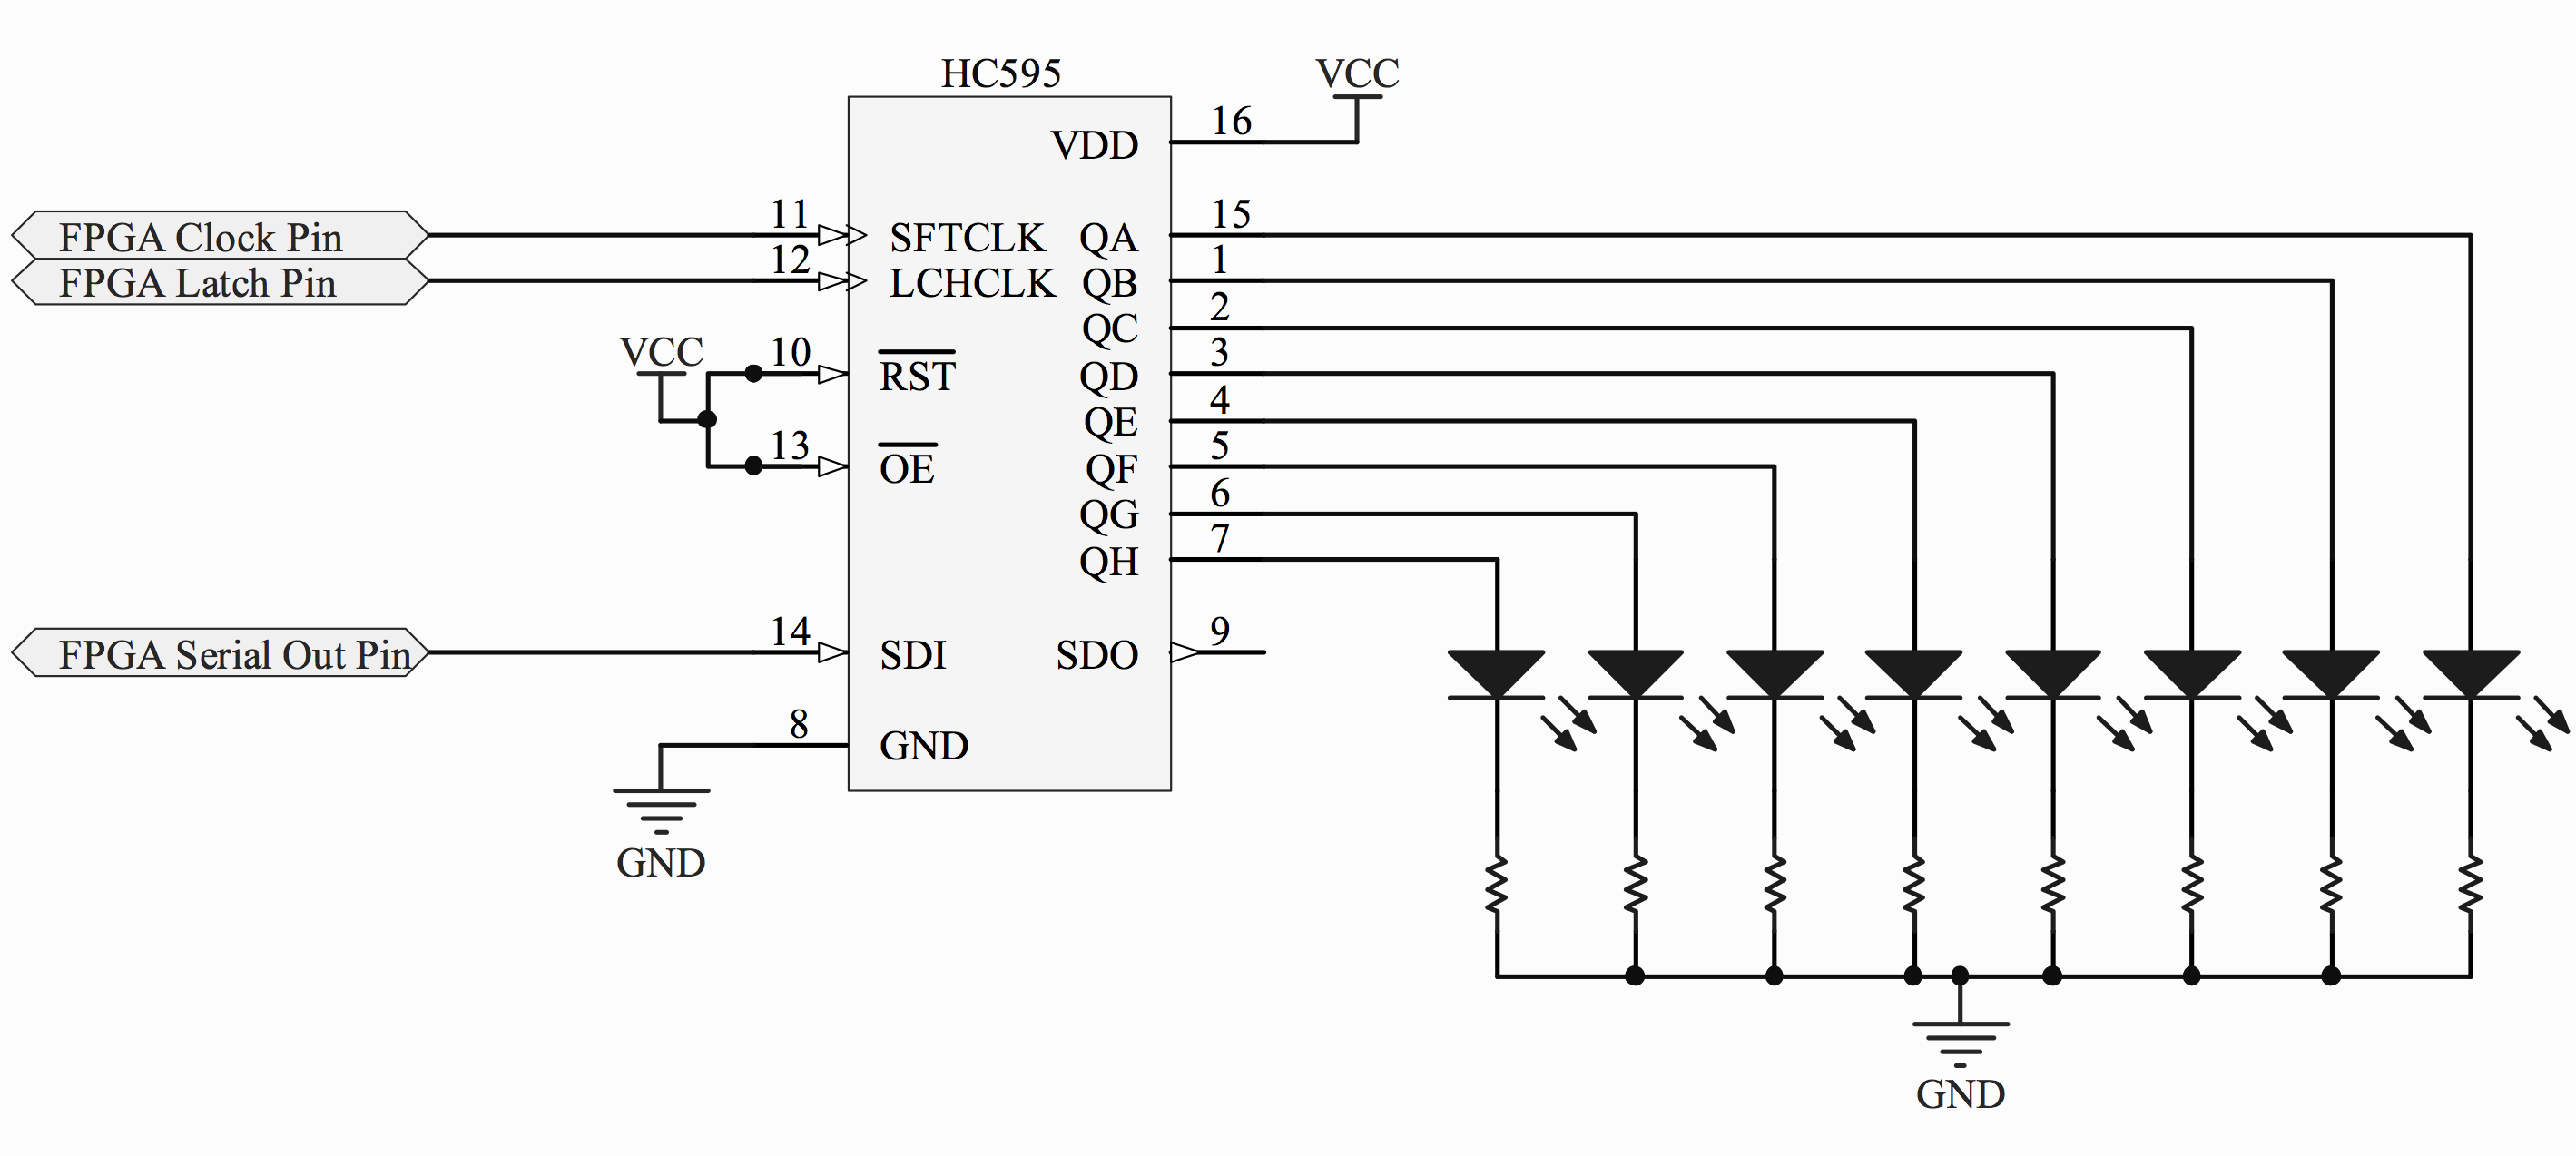
\includegraphics[width=.48\textwidth]{Schematics/ShiftRegister.png}
      \caption{Example application of 595 Shift Register}
      \label{SR}
    \end{figure}

    %| Required Lab Demo
    %| =================================================================================================
    \demo{IO Expansion with Shift Register}
      {Use External DIP switches for 8-bit input and control 8 LEDs attached to a Shift Register though a serial line.}
      {DE0-Nano configured with Comparitor, Clean timing report from TimeQuest}
      {Output LEDs will be inspected for proper operation as the student cycles through the inputs}

%| =================================================================================================
%| Lab Report Requirements
%| =================================================================================================
\section{\bfseries  Lab Report}
    \IEEEPARstart{T}{he} writeup for this lab should be fairly short. This particular lab report will require:
    \subsection{figures to include}
    \begin{itemize}
      \item SignalTap captures for the function generator and shift register.
      \item Code listings for the function generator and shift register
      \item Netlist schematics from the Quartus RTL Netlist viewer.
    \end{itemize}

    \subsection{Questions to Answer}
      \begin{enumerate}
        \item The quartus timing analyzer will report a maximum operating frequency for a circuit. This is dictated by how your design synthesizes and the technology of the FPGA. Can you find the maximum operating frequency of your circuit. \href{http://quartushelp.altera.com/12.1/mergedProjects/analyze/sta/sta_com_report_fmax.htm}{*hint*}
      \end{enumerate}

%| =================================================================================================
%| Conclusions
%| =================================================================================================
\section{\bfseries  Conclusion}
  \IEEEPARstart{L}{ab} four introduced some very important topics. Most applications for FPGA devices will involve frequency requirements that create very difficult timing problems to solve. This is another area where practicing a skill can have a direct effect on employability. The shift register demo is very similar to the implementation of a {\it Serial Periphrial Interface} or SPI in industry. Almost all periphrial devices (Sensors, ADCs, DACs, ...) offer the SPI bus to interact with a control device.

%| =================================================================================================
%| Bibliography
%| =================================================================================================
\bibliographystyle{IEEEtran}
\bibliography{IEEEfull}


\end{document}